% !TEX root = ../../thesis.tex

% Photo Yves Gellie
\cleartoleftpage
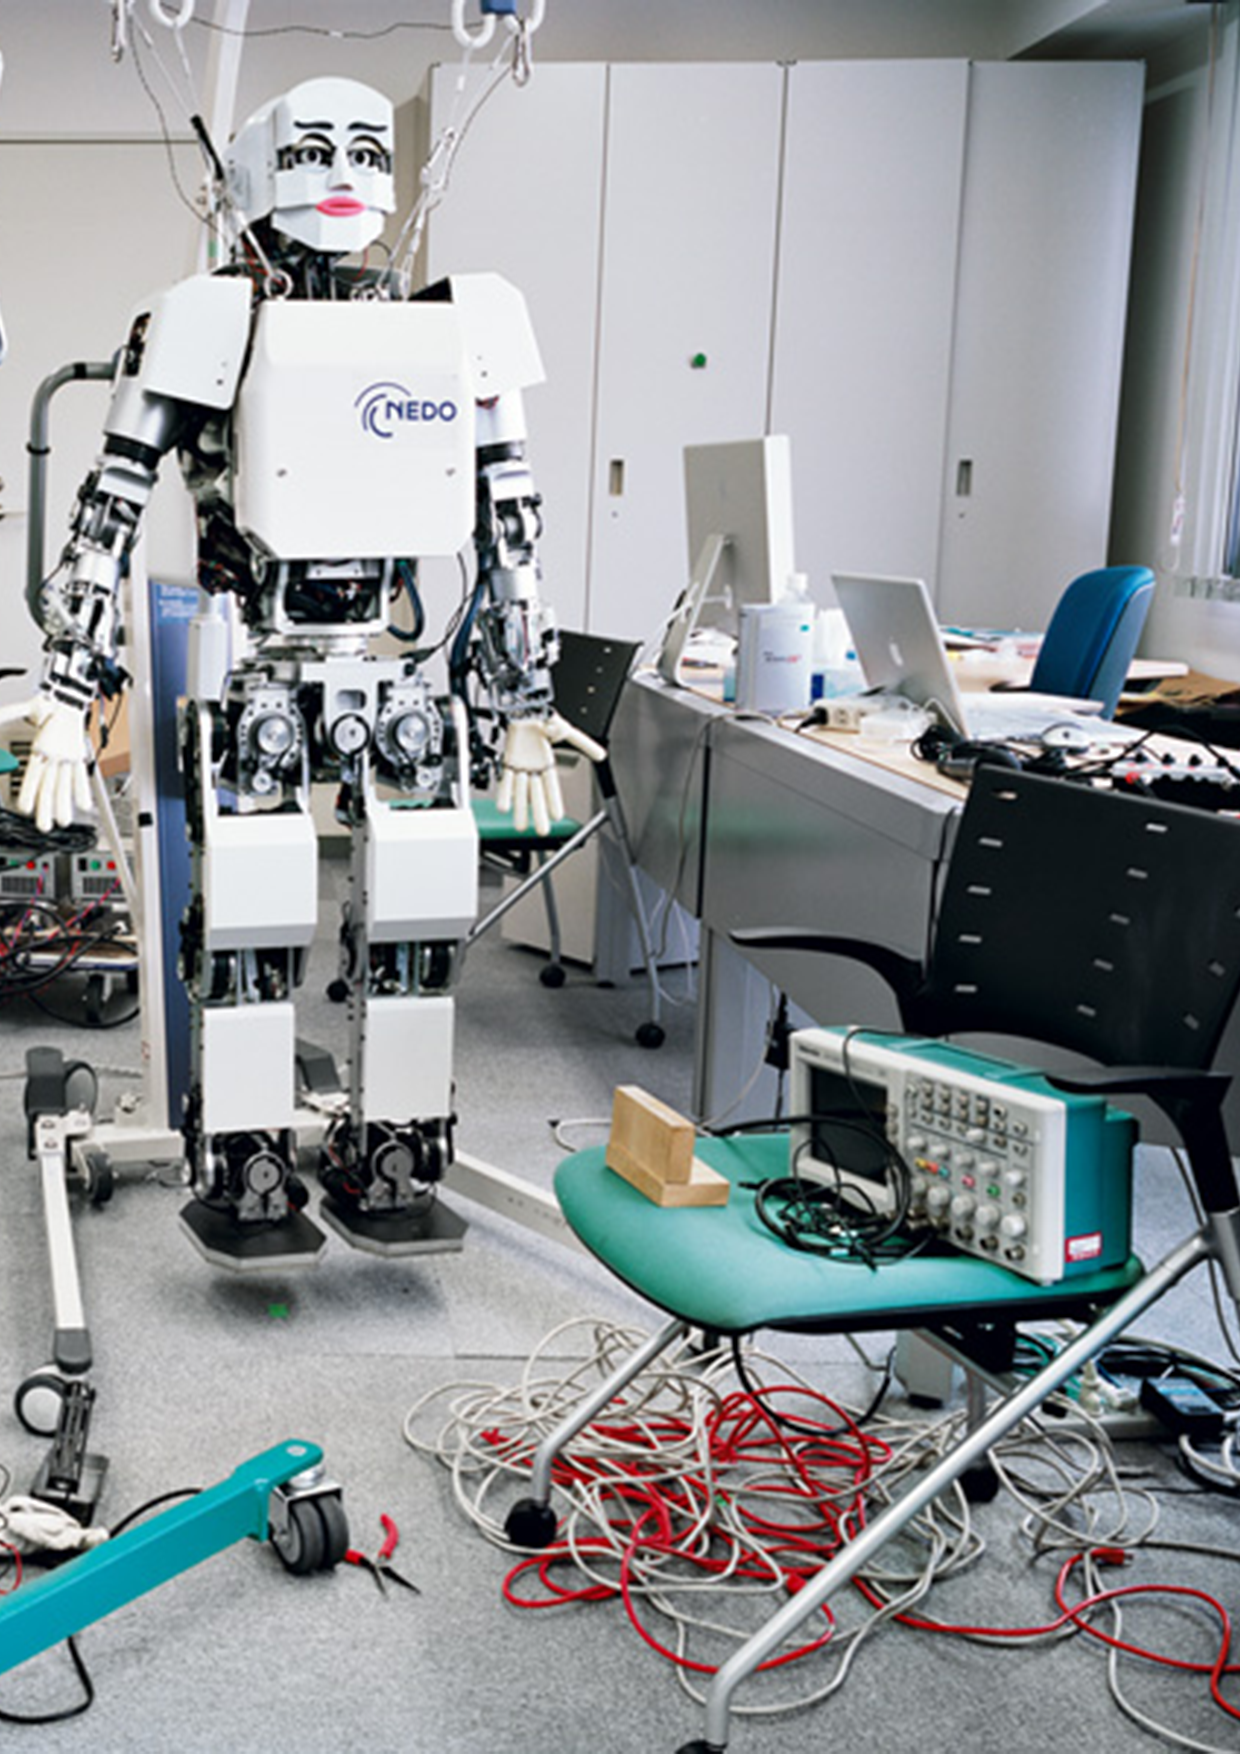
\includepdf{../media/chapter_illustration/robot_setup.pdf}
\chapter{Review of experimental methods} % (fold)
\label{cha:experimental-methods}
\cleanchapterquote{The world is its own best model}{Rodney Brooks}


\section{Introduction} % (fold)

%Context
As we saw it in the previous chapter REF, an interesting evolution of the last decades is the demonstration of the importance of the morphology for sensorimotor control, cognition and development. The role of the morphology appears as a fascinating open field. Exploring the interaction between body properties and cognition could lead to both a better understanding of animals’ behaviour (human being in particular) and to build robot more adapted and robust to an open environment with unpredictable interaction.


%Needs
However as Rodney Brooks explained, exploring interaction between morphology, cognition and environnement requires real world experimentations. Indeed embodiement artificial intelligence REF needs to act in the real world to permit the emergence of complex behavior. The real world includes a large amount of constraints such as inertia, multi-point physical contacts, unpredictable environnement or friction which are, at this time, too complicated to be modeled in physical simulator. Actually "The world is its own best model" and if we can use simulation for exploring basic concepts, the exploration of emergent complex behavior based on interaction between robot self-dynamics and the environment can only be done through experimentation with real robot in real world.

Moreover, as Luc Steels explained (REF), the actual behavior of a robot cannot be programmed. Indeed, its behavior is emerging from the interaction between the controller, the morphology and the environment. Some could argue that adding actual morphology and ecological niche add unnecessary complexity to a problem we already have difficulty to solve by just taking care of the control. Yet it appears some behaviors cannot be achieved without the real physic complexity. A brilliant example are the passive/semi-passive walking robots (presented in sec REF). These robots are technically rather simple, just composed by a mechanical structure with proper link size and foot shape, the establishment of a model should be rather easy but their real dynamic is very difficult to simulate on a physical simulator. Indeed, all complex physic effects (e.g. shocks, friction, inertia) contribute to the achievement of a passive walking.

One of the best state of the art in this domain is the work done by Delft with the different passive and semi passive walkers they built (REF). Desiring to explore biped locomotion with Poppy, we had a discussion with Martijn Wisse on simulation strategy to add semi-passive abilities to Poppy. Here is his his testimony when they try to make their robot walk in simulation after managing to create the real one:

\begin{formal}

Even after obtaining a successful walking motion, we did not manage to create a simulation that walked successfully using the same controller parameters. We tried very hard with some of the best people, but we didn’t succeed. The reason was, I think, that our type of control (using the emergent behavior of a set of simple reflex-like controllers) was highly sensitive to hardware effects like friction. Normally, one uses a local joint controller to make the joint follow a desired trajectory independent of the exact amount of friction. The local controller "abstracts these hardware effects away", if you know what I mean. This makes the behavior of the whole system quite predictable. However, in our robots, we did not have this kind of abstraction as we were not following trajectories, and thus a little bit of extra friction has an effect on the entire motion.

We did spend a long time making a high-fidelity model in Adams, and also using other methods, but eventually we gave up without success.

\signed{Martijn Wisse - Associate professor at Delft University of Technology}
\end{formal}

Thus the results we can find in simulator are very limited and experiments in the real world are needed to

We could say the simulator is indeed a bad idea for low-level control but is suitable for exploring high-level, yet there is no reason the real world does not act the same way on high level control. And it is probable the constraints of the real world can somehow guide the path.

Thus it appears essential to have real robotic platforms to explore role of morphology on control but also highly probable it can have a strong impact when ones are interested by exploring more high-level process (e.g. A.I) ~\parencite{lakoff2000mathematics}.


%objet
In this chapter, we will review the current state of the art in experimental robotic platforms (see REF). Then we will see how current researcher create robot to explore morphological properties.

There are plenty of robotics platforms, from robot arm (Jako, LWR, Kuka) to wheeled platform (Pioneer 3-AT, P3-DX) or even submarine (AQUA2). However, in this Phd thesis we are particulary interested by the locomotion so we will restraint the review to bipedal platform.


\section{section name} % (fold)
\label{sec:section_name}

% section section_name (end)


\section{Affordable humanoid platform} % (fold)
\label{sec:affordable_humanoid_platform}

Other current research platforms are easily accessible and easy to use such as Nao \cite{gouaillier2008nao}, Darwin Op \cite{ha2011development}, Nimbro Op \cite{schwarznimbro} or iCub \cite{metta2008icub}.

\begin{figure}[tb]
\centering
    \subfloat[][Darmin Op]{\label{fig:darwin-op}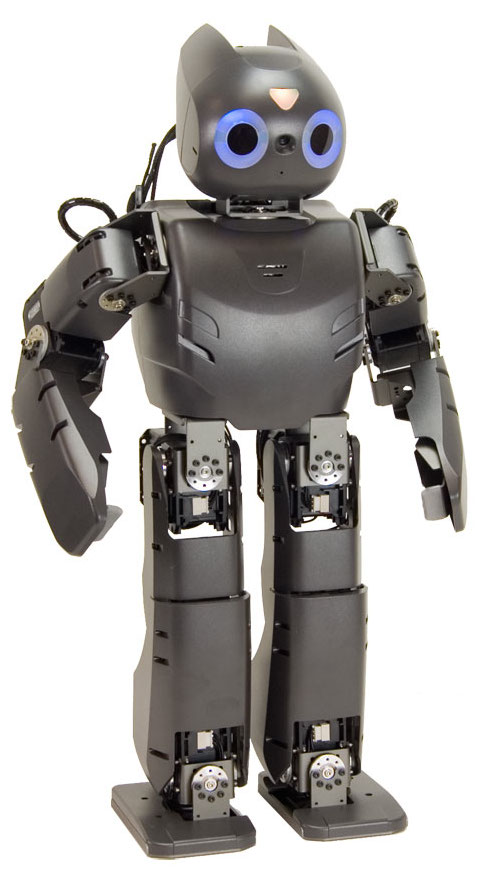
\includegraphics[height=6.5cm]{darwin_op_face.jpg}}
    \hfil
    \subfloat[][Nao]{\label{fig:Nao}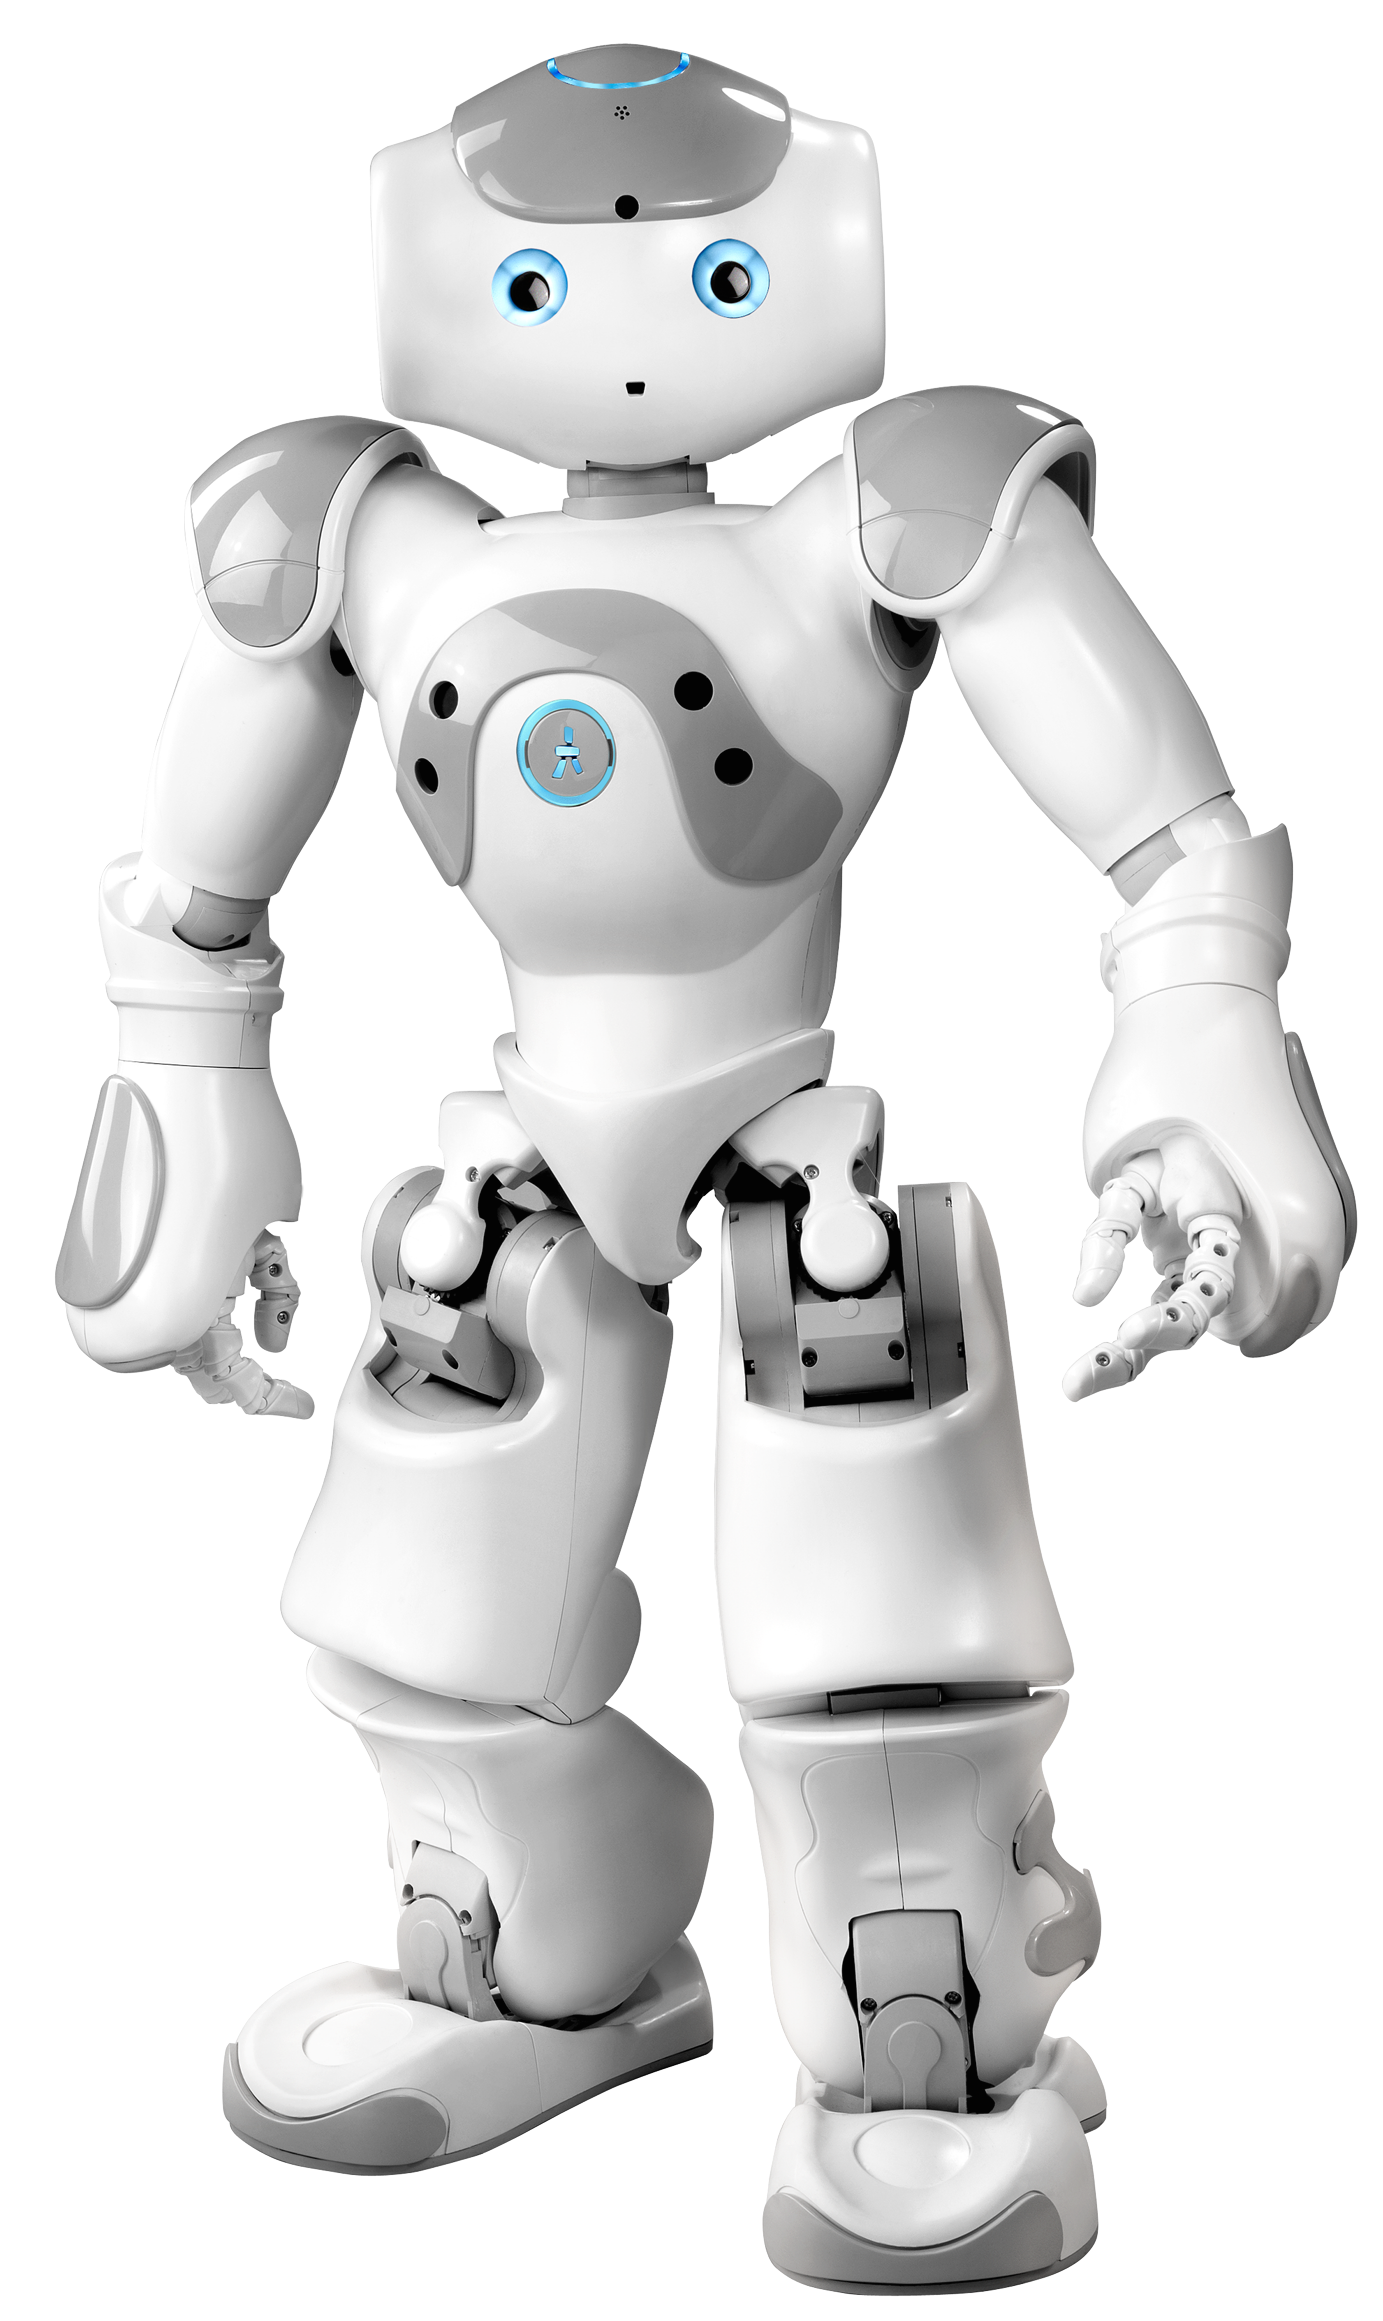
\includegraphics[height=6.5cm]{nao_face.png}}
    \hfil
    \subfloat[][Nimbro OP]{\label{fig:nimbro-op}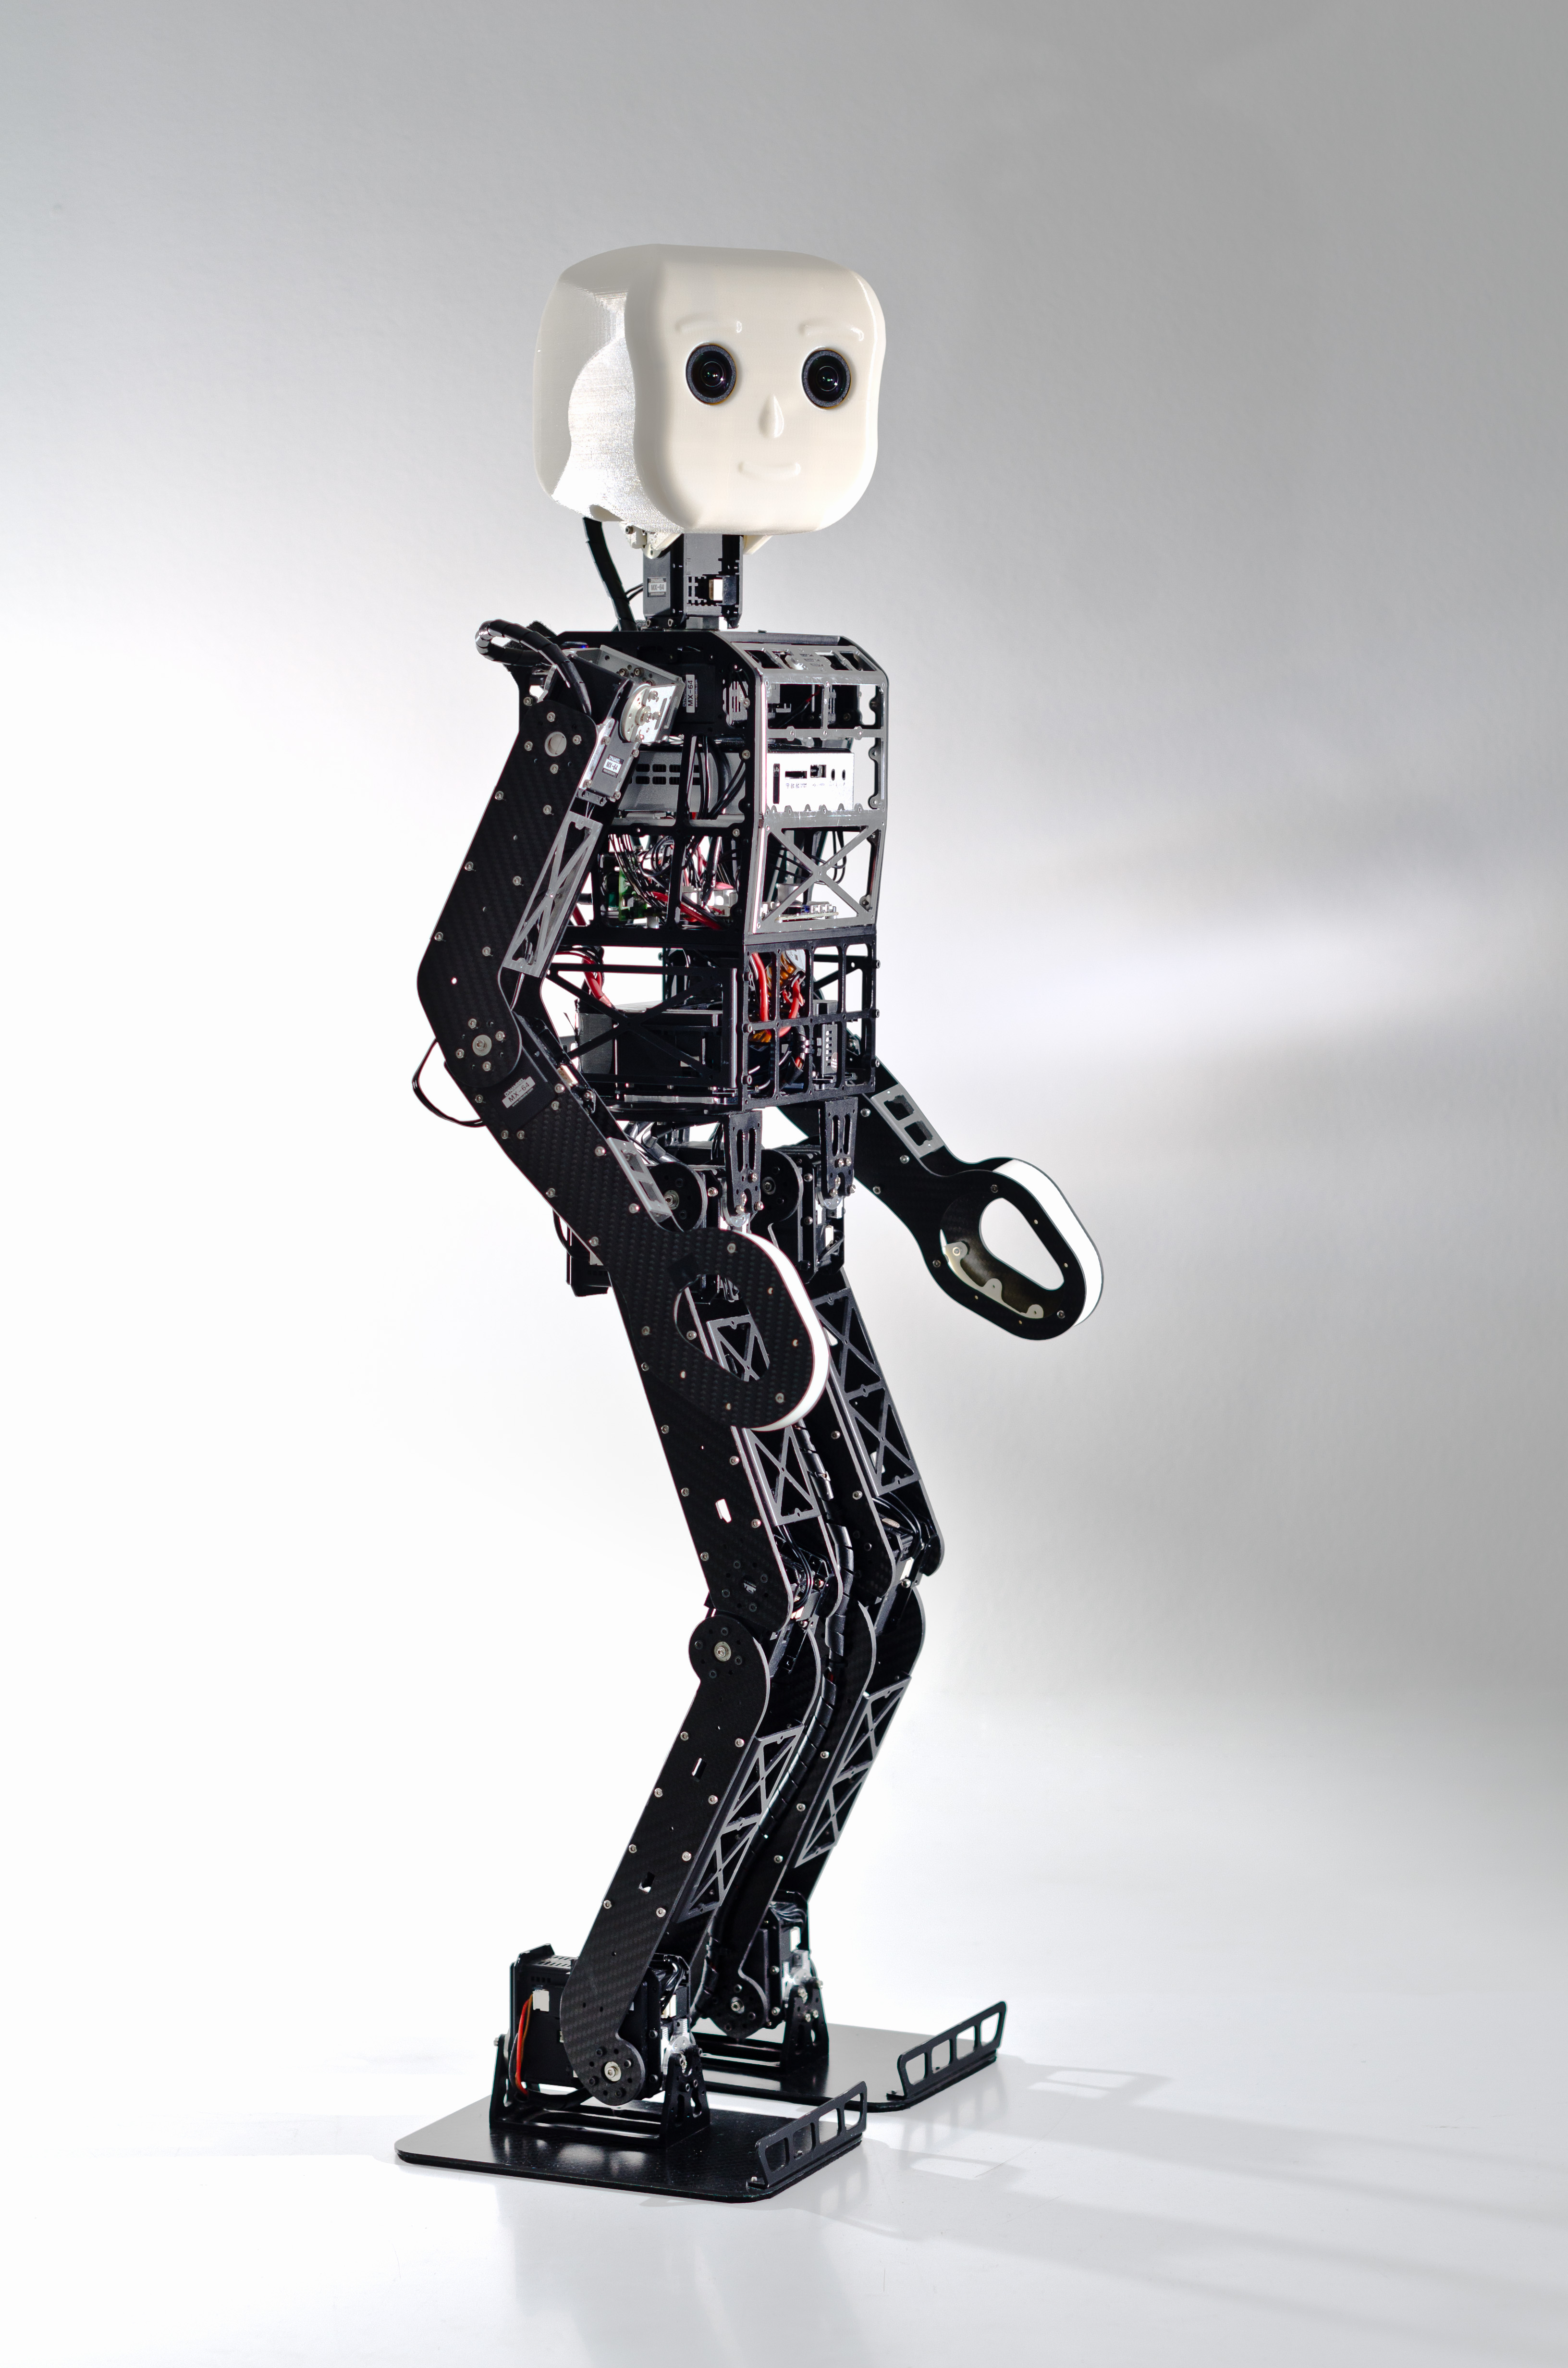
\includegraphics[height=6.5cm]{nimbro-op_1.jpg}}
    \caption{Three humanoid robots made by KumoTek (USA).}
    \label{fig:kumotek_robots}
\end{figure}


\begin{description}
    \item[DARwIn Op] is an open source humanoid research platform created by the Romela lab at Virginia tech~\parencite{ha2011development} and distributed by Robotis for about \$12,000 (see \figurename~\ref{fig:darwin-op}). It measures 45cm height, weights 2.9kg, and has 20 Dynamixel MX-28 actuators (6 for each leg, 3 for each arm, and 2 for the neck). Its mechanical structure is composed by aluminum parts.
    \item[Nao] is 55cm height, 5.2kg and 25DoFs humanoid robot with a plastic mechanical structure (ABS,PA,XCF) (see \figurename~\ref{fig:Nao}). It is a very famous robot sold by few thousands units to labs and universities. Its cost was around \texteuro12,000, but recently it was reduced by half.
    \item[Nimbro-OP] is a tall humanoid with 95cm and 6.6 kg, it has 20 powerful MX-106 and MX-64 actuators (6 per leg, 3 per arm and 2 in the neck). It costs \$20,000 and its structure is based on aluminum and carbon composite (see \figurename~\ref{fig:nimbro-op}).
\end{description}

Yet, they provide a "traditional" morphology (e.g. limited compliance, rigid torso, big feet, over actuated) which can not be easily modified. It makes them unadapted to study the impact of the morphology on biped locomotion and human physical interaction.



\section{Modular robotics} % (fold)

Despite all robotic platform developed, there are only few allowing a complete reconfiguration of their hardware design.

We can find some modular robots examples such as Molecubes~\parencite{zykov2007molecubes}, M-Tran~\parencite{murata2002m}, Superbot~\parencite{salemi2006superbot}, ATRON~\parencite{jorgensen2004modular} or Roombots~\parencite{sproewitz2009roombots}. They are independent robot modules, which can be assembled together to create various robot form and applications (see \figurename~\ref{fig:modular-robots}). However, this kind of robot are not suitable to explore morphological properties and to create humanoid robots.

\begin{figure}[tb]
\centering
    \subfloat[][ATRON]{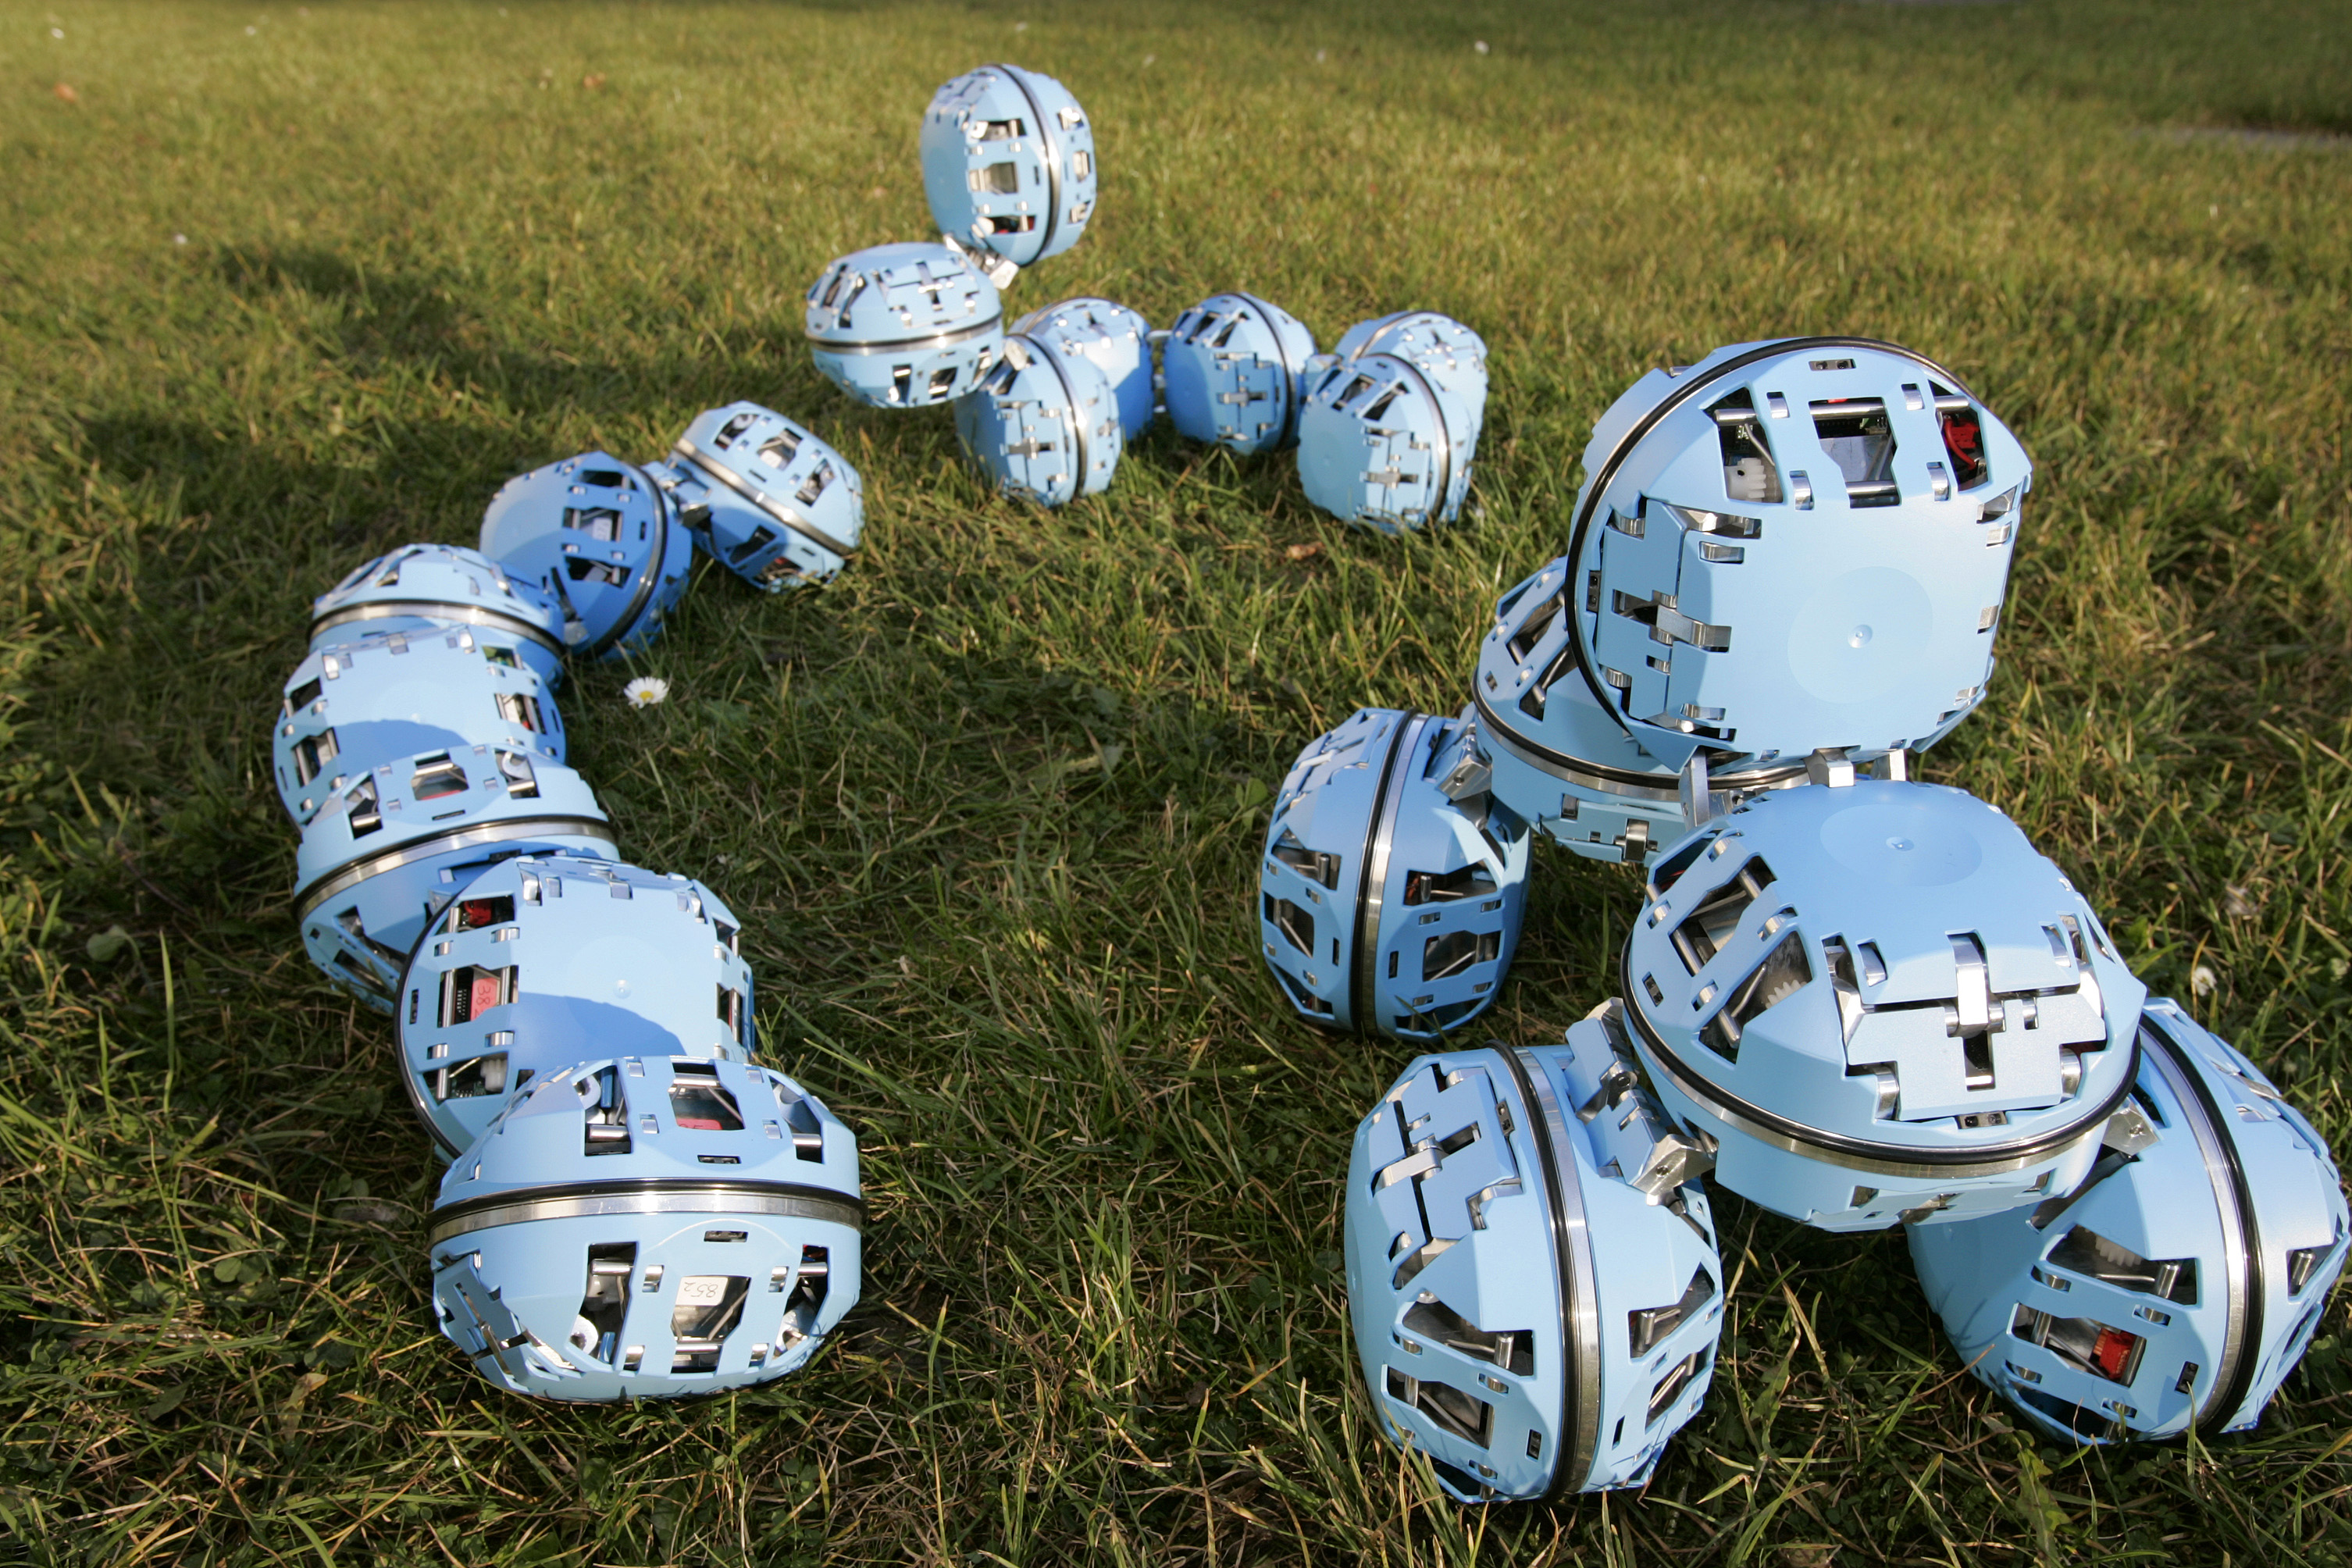
\includegraphics[width=0.45\linewidth]{ATRON.jpg}}
    \hfil
    \subfloat[][Roombots]{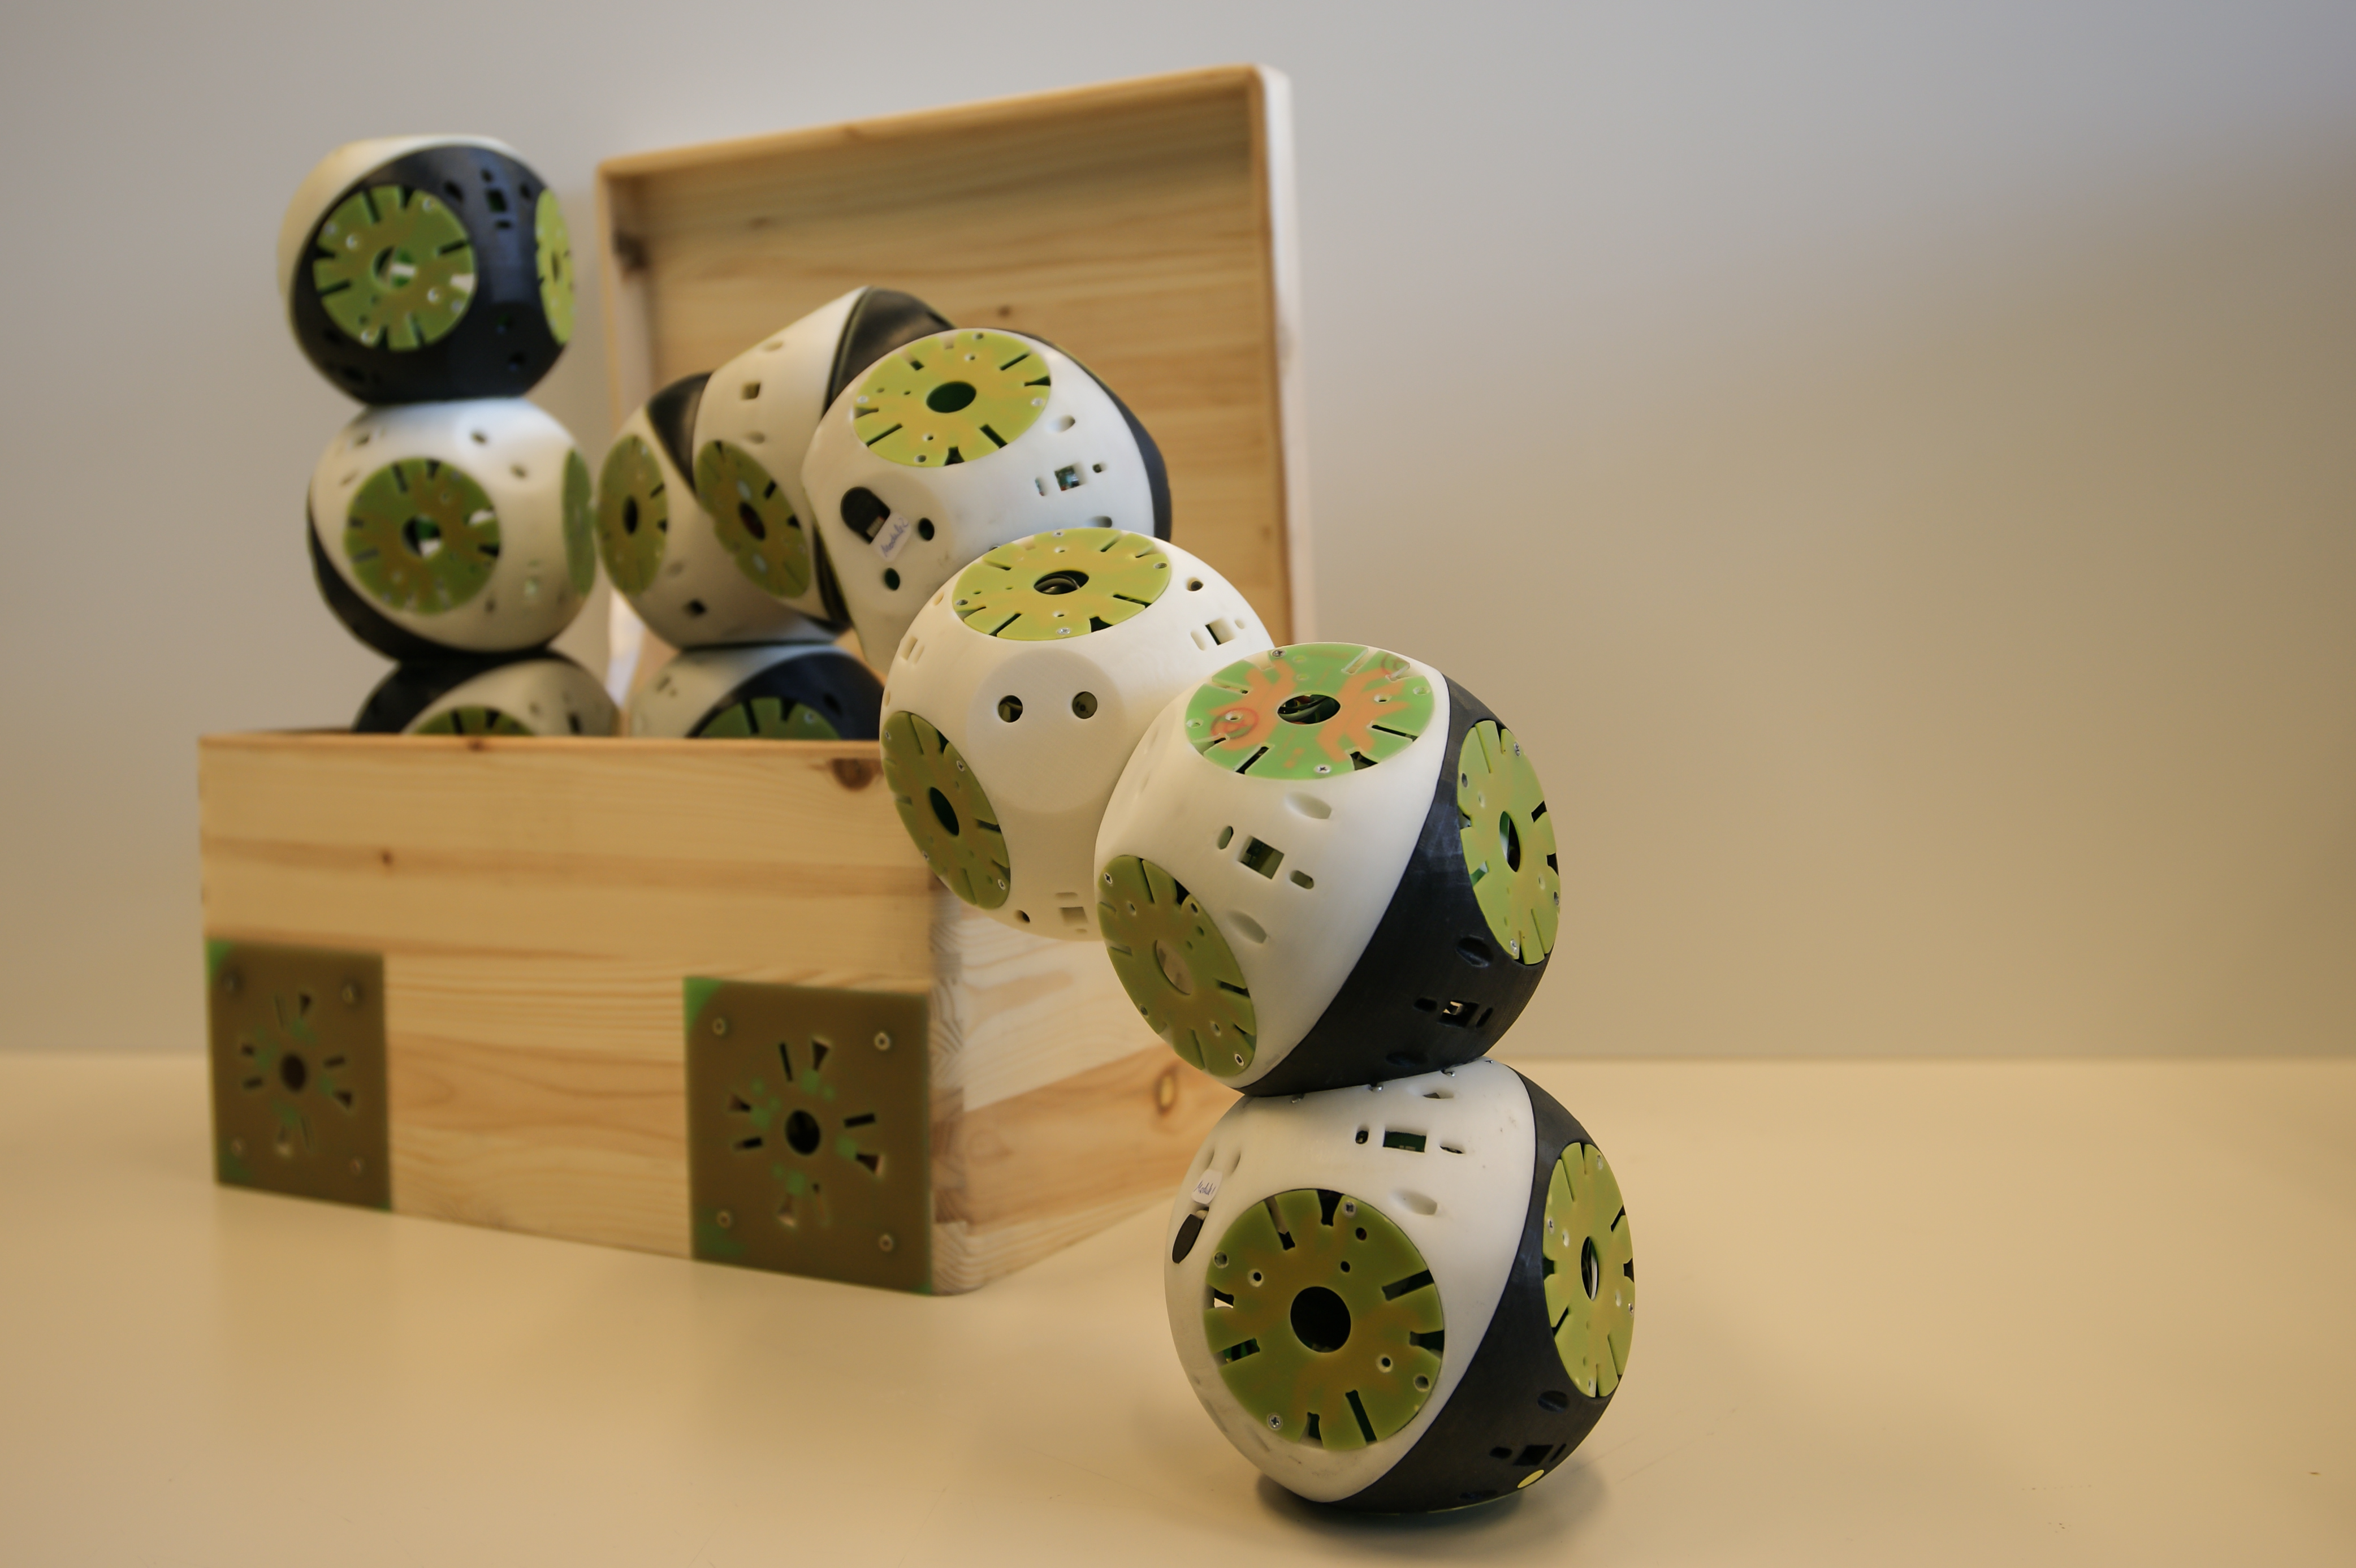
\includegraphics[width=0.45\linewidth]{roombots.jpg}}
    \caption{Modular robots}
    \label{fig:modular-robots}
\end{figure}

Actually, to our best knowledge there is only one example of modular kit allowing to really explore the role of morphology. The Locomorph project~\parencite{locomorph} offers a multi-purpose hardware kit called LocoKit~\parencite{larsen2012locokit}). This kit uses carbon-fiber rods assembled with Locokit parts (see \figurename~\ref{fig:locokit-parts}). It allows quickly creating robot and studying the impact of several morphological properties such as link length, joint stiffness or mass distribution (see \figurename~\ref{fig:locokit}). Also it permits to add spring over rods to create linear damping system and therefore add compliance to robots.
The kit is distributed for \texteuro2500 and include the needed components to create a quadruped robot (see \figurename~\ref{fig:locokit-example}).

\begin{figure}[tb]
\centering
    \subfloat[][]{\label{fig:locokit-parts}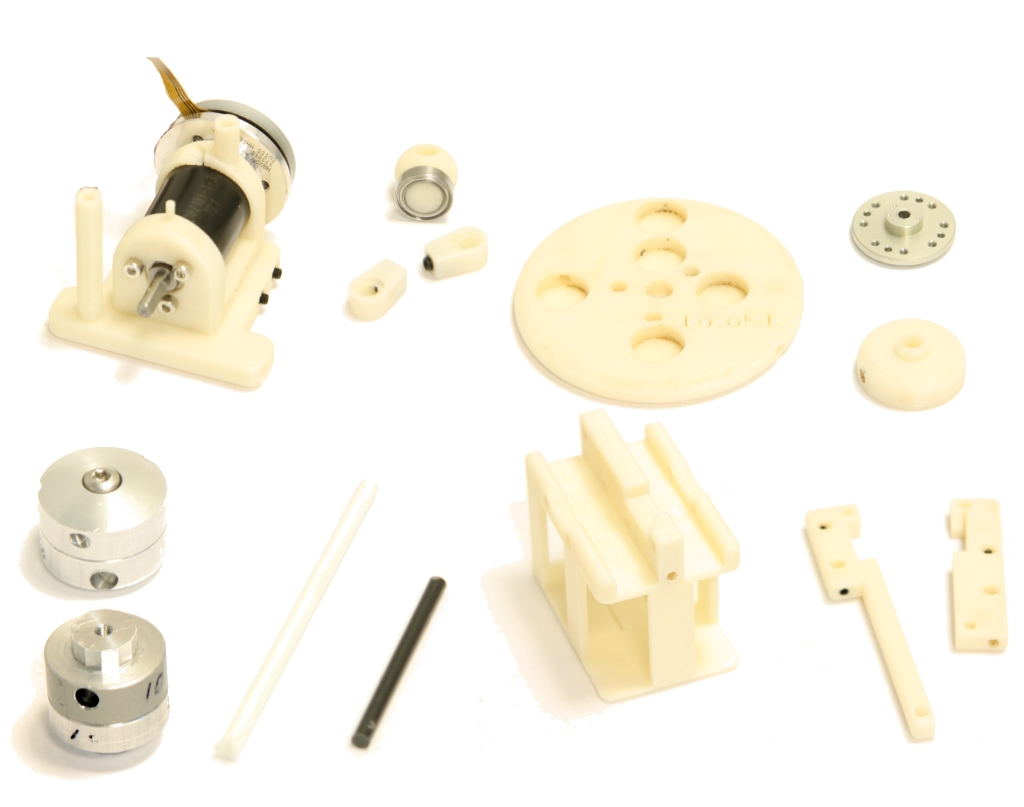
\includegraphics[height=5cm]{locokit-parts.jpg}}
    \hfil
    \subfloat[][]{\label{fig:locokit-example}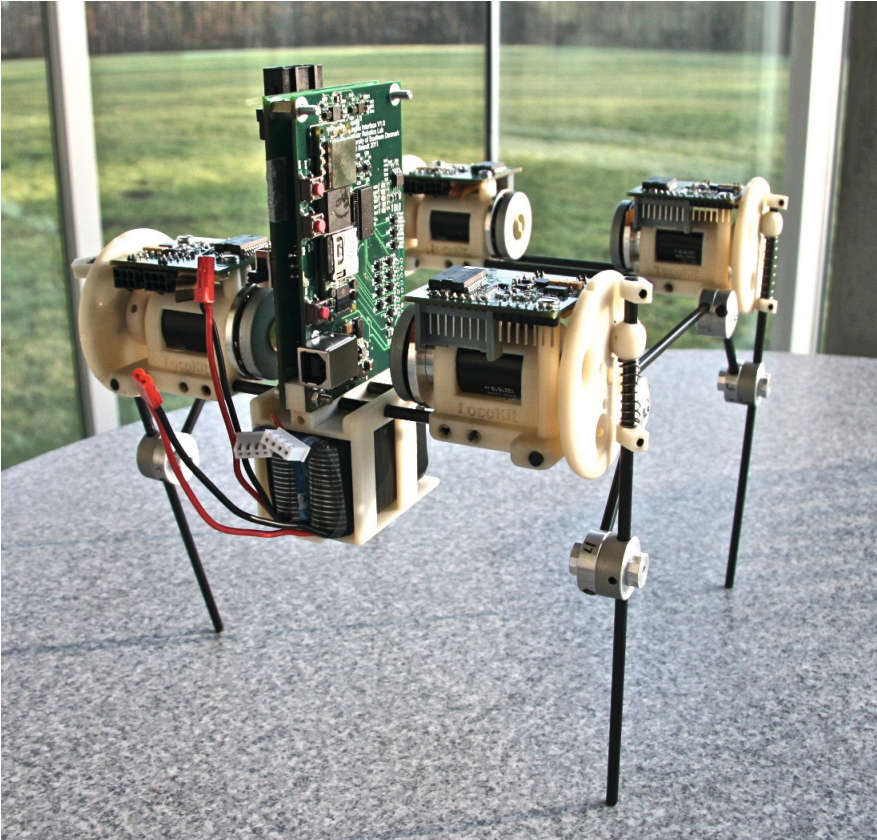
\includegraphics[height=5cm]{locokit-example.png}}
    \caption{}
    \label{fig:locokit}
\end{figure}

It appears as the only existing solution allowing to both explore the role of morphology and transfer results between laboratory. While being very interesting, it is also limited as it implies to create rods-based robot and multi-body articulation such as ones we can find in a human leg or trunk seem complicated to produce.


\section{Conclusion}

In the previous chapter, we presented several work showing the importance of the robot morphology and the need to continue the research in this domain. As we explained in the introduction see REF, this research requires to have real robotic platform to be explored.


On one hand, some robotic platforms such as Denise or Athlete robot were designed for this purpose and actually shown great results about the role of passive dynamic or compliance on biped walking. However, these platform are prototypes produced specifically for a lab and are nearly impossible to reproduce on another lab.
In addition, while they use classical production technique with metal casting, they are quite complex and expensive to modify.

On the other hand, commercial robots are easily accessible so the results should be reproducible from one lab to another. Yet their design method involved also classical production techniques, therefore modifying their morphology would require a lot of



In the next chapter, we will present novel production techniques and diffusion ways, which can solve both problem considering exploring the role of morphology and reproducibility between research labs.


However, we saw that none of the available commercial robot platform permits such scientific exploration.

Also, the current research practices in the Robotics field limit the diffusion and the impact of contributions.
Indeed, in most cases, there is no material associated with a published paper.
Meaning, only the theory is shared with the community but not the actual framework allowing to reproduce the results.

% \begin{itemize}
%     \item Lost of time, design a whole new robot.
%     \item Morphology as an experimental variable
%     \item Current robotic platforms do not permit to explore the morphology as a variable.
%     \item IA haut niveau qui peut se faire en simulation avec certaines reserves.
%     \item Currently, robot platform are not satisfying if we want to explore the role of morphology.
%     They are not hackable and proto or not both easy to use and accessible.
%     \item Problem with simulator VS real world
%     \item Exploring control with real robot raise challenge due to error
%     \item Morphologie as variable experimental
%     \item Engineering on the platform not research
%     \item There is two categories, commercial platform and research lab prototype.
%     \item No distribution of the code
%     \item no benchmark platform
%     \item no hackable platform
% \end{itemize}

% This raises limitations for:
% \begin{itemize}
%     \item verifying the quality of the results presented in the paper,
%     \item the reuse of the contribution as there is, in most case, a gap between the theory and the actual implementation,
%     \item the collaborative work with other laboratory
% \end{itemize}




